\documentclass[1p]{elsarticle_modified}
%\bibliographystyle{elsarticle-num}

%\usepackage[colorlinks]{hyperref}
%\usepackage{abbrmath_seonhwa} %\Abb, \Ascr, \Acal ,\Abf, \Afrak
\usepackage{amsfonts}
\usepackage{amssymb}
\usepackage{amsmath}
\usepackage{amsthm}
\usepackage{scalefnt}
\usepackage{amsbsy}
\usepackage{kotex}
\usepackage{caption}
\usepackage{subfig}
\usepackage{color}
\usepackage{graphicx}
\usepackage{xcolor} %% white, black, red, green, blue, cyan, magenta, yellow
\usepackage{float}
\usepackage{setspace}
\usepackage{hyperref}

\usepackage{tikz}
\usetikzlibrary{arrows}

\usepackage{multirow}
\usepackage{array} % fixed length table
\usepackage{hhline}

%%%%%%%%%%%%%%%%%%%%%
\makeatletter
\renewcommand*\env@matrix[1][\arraystretch]{%
	\edef\arraystretch{#1}%
	\hskip -\arraycolsep
	\let\@ifnextchar\new@ifnextchar
	\array{*\c@MaxMatrixCols c}}
\makeatother %https://tex.stackexchange.com/questions/14071/how-can-i-increase-the-line-spacing-in-a-matrix
%%%%%%%%%%%%%%%

\usepackage[normalem]{ulem}

\newcommand{\msout}[1]{\ifmmode\text{\sout{\ensuremath{#1}}}\else\sout{#1}\fi}
%SOURCE: \msout is \stkout macro in https://tex.stackexchange.com/questions/20609/strikeout-in-math-mode

\newcommand{\cancel}[1]{
	\ifmmode
	{\color{red}\msout{#1}}
	\else
	{\color{red}\sout{#1}}
	\fi
}

\newcommand{\add}[1]{
	{\color{blue}\uwave{#1}}
}

\newcommand{\replace}[2]{
	\ifmmode
	{\color{red}\msout{#1}}{\color{blue}\uwave{#2}}
	\else
	{\color{red}\sout{#1}}{\color{blue}\uwave{#2}}
	\fi
}

\newcommand{\Sol}{\mathcal{S}} %segment
\newcommand{\D}{D} %diagram
\newcommand{\A}{\mathcal{A}} %arc


%%%%%%%%%%%%%%%%%%%%%%%%%%%%%5 test

\def\sl{\operatorname{\textup{SL}}(2,\Cbb)}
\def\psl{\operatorname{\textup{PSL}}(2,\Cbb)}
\def\quan{\mkern 1mu \triangleright \mkern 1mu}

\theoremstyle{definition}
\newtheorem{thm}{Theorem}[section]
\newtheorem{prop}[thm]{Proposition}
\newtheorem{lem}[thm]{Lemma}
\newtheorem{ques}[thm]{Question}
\newtheorem{cor}[thm]{Corollary}
\newtheorem{defn}[thm]{Definition}
\newtheorem{exam}[thm]{Example}
\newtheorem{rmk}[thm]{Remark}
\newtheorem{alg}[thm]{Algorithm}

\newcommand{\I}{\sqrt{-1}}
\begin{document}

%\begin{frontmatter}
%
%\title{Boundary parabolic representations of knots up to 8 crossings}
%
%%% Group authors per affiliation:
%\author{Yunhi Cho} 
%\address{Department of Mathematics, University of Seoul, Seoul, Korea}
%\ead{yhcho@uos.ac.kr}
%
%
%\author{Seonhwa Kim} %\fnref{s_kim}}
%\address{Center for Geometry and Physics, Institute for Basic Science, Pohang, 37673, Korea}
%\ead{ryeona17@ibs.re.kr}
%
%\author{Hyuk Kim}
%\address{Department of Mathematical Sciences, Seoul National University, Seoul 08826, Korea}
%\ead{hyukkim@snu.ac.kr}
%
%\author{Seokbeom Yoon}
%\address{Department of Mathematical Sciences, Seoul National University, Seoul, 08826,  Korea}
%\ead{sbyoon15@snu.ac.kr}
%
%\begin{abstract}
%We find all boundary parabolic representation of knots up to 8 crossings.
%
%\end{abstract}
%\begin{keyword}
%    \MSC[2010] 57M25 
%\end{keyword}
%
%\end{frontmatter}

%\linenumbers
%\tableofcontents
%
\newcommand\colored[1]{\textcolor{white}{\rule[-0.35ex]{0.8em}{1.4ex}}\kern-0.8em\color{red} #1}%
%\newcommand\colored[1]{\textcolor{white}{ #1}\kern-2.17ex	\textcolor{white}{ #1}\kern-1.81ex	\textcolor{white}{ #1}\kern-2.15ex\color{red}#1	}

{\Large $\underline{11a_{64}~(K11a_{64})}$}

\setlength{\tabcolsep}{10pt}
\renewcommand{\arraystretch}{1.6}
\vspace{1cm}\begin{tabular}{m{100pt}>{\centering\arraybackslash}m{274pt}}
\multirow{5}{120pt}{
	\centering
	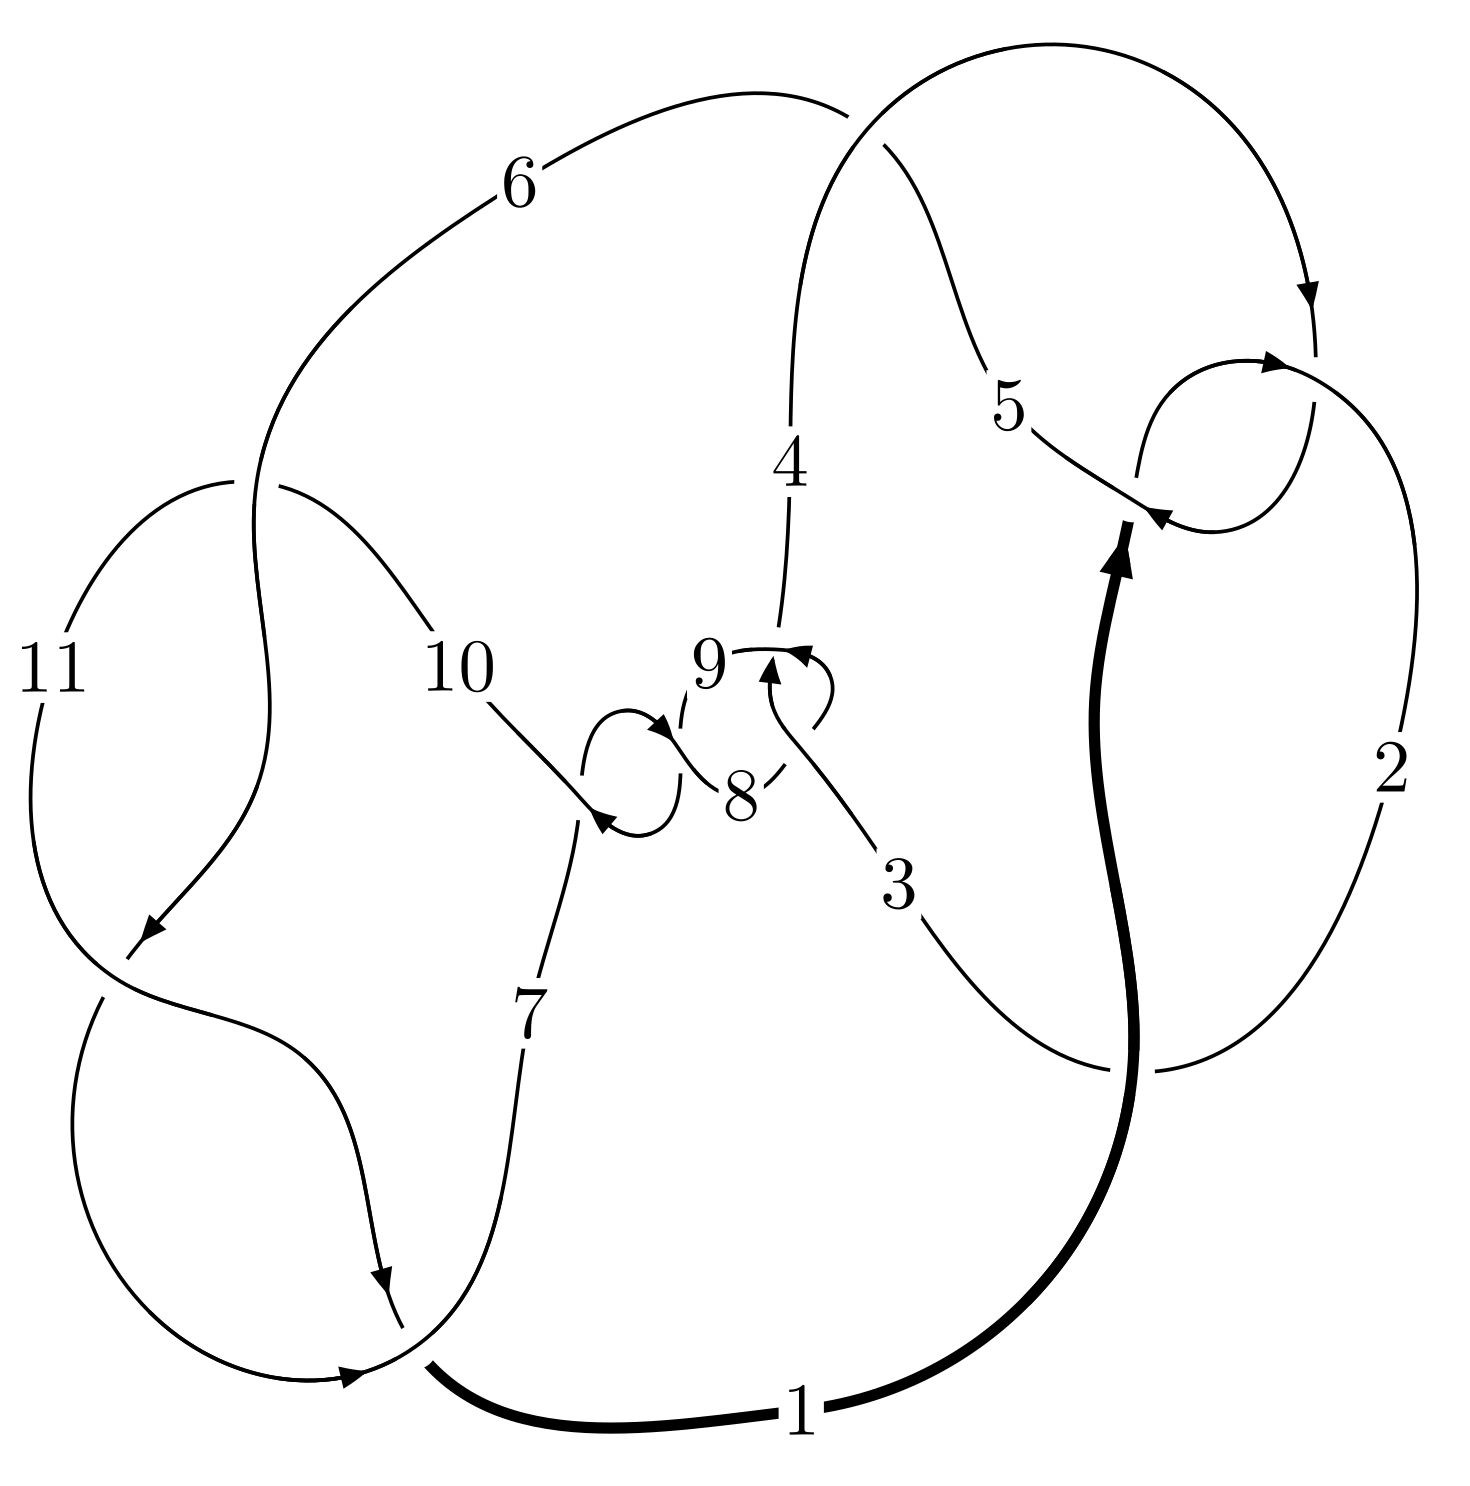
\includegraphics[width=112pt]{../../../GIT/diagram.site/Diagrams/png/313_11a_64.png}\\
\ \ \ A knot diagram\footnotemark}&
\allowdisplaybreaks
\textbf{Linearized knot diagam} \\
\cline{2-2}
 &
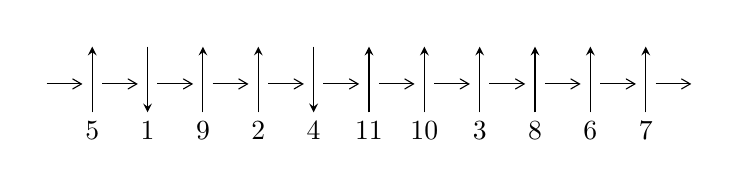
\begin{tikzpicture}[x=20pt, y=17pt]
	% nodes
	\node (C0) at (0, 0) {};
	\node (C1) at (1, 0) {};
	\node (C1U) at (1, +1) {};
	\node (C1D) at (1, -1) {5};

	\node (C2) at (2, 0) {};
	\node (C2U) at (2, +1) {};
	\node (C2D) at (2, -1) {1};

	\node (C3) at (3, 0) {};
	\node (C3U) at (3, +1) {};
	\node (C3D) at (3, -1) {9};

	\node (C4) at (4, 0) {};
	\node (C4U) at (4, +1) {};
	\node (C4D) at (4, -1) {2};

	\node (C5) at (5, 0) {};
	\node (C5U) at (5, +1) {};
	\node (C5D) at (5, -1) {4};

	\node (C6) at (6, 0) {};
	\node (C6U) at (6, +1) {};
	\node (C6D) at (6, -1) {11};

	\node (C7) at (7, 0) {};
	\node (C7U) at (7, +1) {};
	\node (C7D) at (7, -1) {10};

	\node (C8) at (8, 0) {};
	\node (C8U) at (8, +1) {};
	\node (C8D) at (8, -1) {3};

	\node (C9) at (9, 0) {};
	\node (C9U) at (9, +1) {};
	\node (C9D) at (9, -1) {8};

	\node (C10) at (10, 0) {};
	\node (C10U) at (10, +1) {};
	\node (C10D) at (10, -1) {6};

	\node (C11) at (11, 0) {};
	\node (C11U) at (11, +1) {};
	\node (C11D) at (11, -1) {7};
	\node (C12) at (12, 0) {};

	% arrows
	\draw[->,>={angle 60}]
	(C0) edge (C1) (C1) edge (C2) (C2) edge (C3) (C3) edge (C4) (C4) edge (C5) (C5) edge (C6) (C6) edge (C7) (C7) edge (C8) (C8) edge (C9) (C9) edge (C10) (C10) edge (C11) (C11) edge (C12) ;	\draw[->,>=stealth]
	(C1D) edge (C1U) (C2U) edge (C2D) (C3D) edge (C3U) (C4D) edge (C4U) (C5U) edge (C5D) (C6D) edge (C6U) (C7D) edge (C7U) (C8D) edge (C8U) (C9D) edge (C9U) (C10D) edge (C10U) (C11D) edge (C11U) ;
	\end{tikzpicture} \\
\hhline{~~} \\& 
\textbf{Solving Sequence} \\ \cline{2-2} 
 &
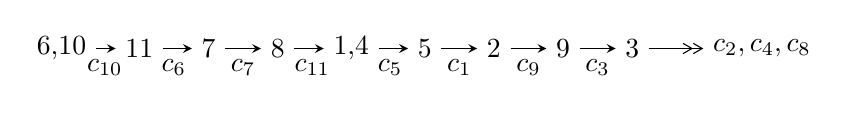
\begin{tikzpicture}[x=25pt, y=7pt]
	% node
	\node (A0) at (-1/8, 0) {6,10};
	\node (A1) at (1, 0) {11};
	\node (A2) at (2, 0) {7};
	\node (A3) at (3, 0) {8};
	\node (A4) at (65/16, 0) {1,4};
	\node (A5) at (41/8, 0) {5};
	\node (A6) at (49/8, 0) {2};
	\node (A7) at (57/8, 0) {9};
	\node (A8) at (65/8, 0) {3};
	\node (C1) at (1/2, -1) {$c_{10}$};
	\node (C2) at (3/2, -1) {$c_{6}$};
	\node (C3) at (5/2, -1) {$c_{7}$};
	\node (C4) at (7/2, -1) {$c_{11}$};
	\node (C5) at (37/8, -1) {$c_{5}$};
	\node (C6) at (45/8, -1) {$c_{1}$};
	\node (C7) at (53/8, -1) {$c_{9}$};
	\node (C8) at (61/8, -1) {$c_{3}$};
	\node (A9) at (10, 0) {$c_{2},c_{4},c_{8}$};

	% edge
	\draw[->,>=stealth]	
	(A0) edge (A1) (A1) edge (A2) (A2) edge (A3) (A3) edge (A4) (A4) edge (A5) (A5) edge (A6) (A6) edge (A7) (A7) edge (A8) ;
	\draw[->>,>={angle 60}]	
	(A8) edge (A9);
\end{tikzpicture} \\ 

\end{tabular} \\

\footnotetext{
The image of knot diagram is generated by the software ``\textbf{Draw programme}" developed by Andrew Bartholomew(\url{http://www.layer8.co.uk/maths/draw/index.htm\#Running-draw}), where we modified some parts for our purpose(\url{https://github.com/CATsTAILs/LinksPainter}).
}\phantom \\ \newline 
\centering \textbf{Ideals for irreducible components\footnotemark of $X_{\text{par}}$} 
 
\begin{align*}
I^u_{1}&=\langle 
-5 u^{49}-9 u^{48}+\cdots+b+4,\;3 u^{49}+4 u^{48}+\cdots+2 a-1,\;u^{50}+3 u^{49}+\cdots+9 u^2-1\rangle \\
I^u_{2}&=\langle 
b,\;a^2- a+1,\;u-1\rangle \\
\\
\end{align*}
\raggedright * 2 irreducible components of $\dim_{\mathbb{C}}=0$, with total 52 representations.\\
\footnotetext{All coefficients of polynomials are rational numbers. But the coefficients are sometimes approximated in decimal forms when there is not enough margin.}
\newpage
\renewcommand{\arraystretch}{1}
\centering \section*{I. $I^u_{1}= \langle -5 u^{49}-9 u^{48}+\cdots+b+4,\;3 u^{49}+4 u^{48}+\cdots+2 a-1,\;u^{50}+3 u^{49}+\cdots+9 u^2-1 \rangle$}
\flushleft \textbf{(i) Arc colorings}\\
\begin{tabular}{m{7pt} m{180pt} m{7pt} m{180pt} }
\flushright $a_{6}=$&$\begin{pmatrix}0\\u\end{pmatrix}$ \\
\flushright $a_{10}=$&$\begin{pmatrix}1\\0\end{pmatrix}$ \\
\flushright $a_{11}=$&$\begin{pmatrix}1\\- u^2\end{pmatrix}$ \\
\flushright $a_{7}=$&$\begin{pmatrix}u\\- u^3+u\end{pmatrix}$ \\
\flushright $a_{8}=$&$\begin{pmatrix}- u^3+2 u\\- u^3+u\end{pmatrix}$ \\
\flushright $a_{1}=$&$\begin{pmatrix}- u^2+1\\u^4-2 u^2\end{pmatrix}$ \\
\flushright $a_{4}=$&$\begin{pmatrix}-\frac{3}{2} u^{49}-2 u^{48}+\cdots+\frac{1}{2} u+\frac{1}{2}\\5 u^{49}+9 u^{48}+\cdots+4 u-4\end{pmatrix}$ \\
\flushright $a_{5}=$&$\begin{pmatrix}\frac{1}{2} u^{49}+u^{48}+\cdots-\frac{11}{2} u+\frac{1}{2}\\- u^{16}+6 u^{14}+\cdots-6 u^3+4 u^2\end{pmatrix}$ \\
\flushright $a_{2}=$&$\begin{pmatrix}\frac{5}{2} u^{49}+4 u^{48}+\cdots+\frac{1}{2} u-\frac{1}{2}\\-\frac{1}{2} u^{49}- u^{48}+\cdots-\frac{1}{2} u+\frac{1}{2}\end{pmatrix}$ \\
\flushright $a_{9}=$&$\begin{pmatrix}u^6-3 u^4+2 u^2+1\\u^6-2 u^4+u^2\end{pmatrix}$ \\
\flushright $a_{3}=$&$\begin{pmatrix}-\frac{9}{2} u^{49}-8 u^{48}+\cdots-\frac{5}{2} u+\frac{5}{2}\\-2 u^{49}-3 u^{48}+\cdots-8 u^2+1\end{pmatrix}$\\ \flushright $a_{3}=$&$\begin{pmatrix}-\frac{9}{2} u^{49}-8 u^{48}+\cdots-\frac{5}{2} u+\frac{5}{2}\\-2 u^{49}-3 u^{48}+\cdots-8 u^2+1\end{pmatrix}$\\&\end{tabular}
\flushleft \textbf{(ii) Obstruction class $= -1$}\\~\\
\flushleft \textbf{(iii) Cusp Shapes $= -18 u^{49}-27 u^{48}+\cdots-2 u+25$}\\~\\
\newpage\renewcommand{\arraystretch}{1}
\flushleft \textbf{(iv) u-Polynomials at the component}\newline \\
\begin{tabular}{m{50pt}|m{274pt}}
Crossings & \hspace{64pt}u-Polynomials at each crossing \\
\hline $$\begin{aligned}c_{1},c_{4}\end{aligned}$$&$\begin{aligned}
&u^{50}+2 u^{49}+\cdots-3 u+1
\end{aligned}$\\
\hline $$\begin{aligned}c_{2},c_{5}\end{aligned}$$&$\begin{aligned}
&u^{50}+18 u^{49}+\cdots+u+1
\end{aligned}$\\
\hline $$\begin{aligned}c_{3},c_{8}\end{aligned}$$&$\begin{aligned}
&u^{50}+u^{49}+\cdots+4 u-4
\end{aligned}$\\
\hline $$\begin{aligned}c_{6},c_{10},c_{11}\end{aligned}$$&$\begin{aligned}
&u^{50}+3 u^{49}+\cdots+9 u^2-1
\end{aligned}$\\
\hline $$\begin{aligned}c_{7},c_{9}\end{aligned}$$&$\begin{aligned}
&u^{50}-15 u^{49}+\cdots-104 u+16
\end{aligned}$\\
\hline
\end{tabular}\\~\\
\newpage\renewcommand{\arraystretch}{1}
\flushleft \textbf{(v) Riley Polynomials at the component}\newline \\
\begin{tabular}{m{50pt}|m{274pt}}
Crossings & \hspace{64pt}Riley Polynomials at each crossing \\
\hline $$\begin{aligned}c_{1},c_{4}\end{aligned}$$&$\begin{aligned}
&y^{50}+18 y^{49}+\cdots+y+1
\end{aligned}$\\
\hline $$\begin{aligned}c_{2},c_{5}\end{aligned}$$&$\begin{aligned}
&y^{50}+30 y^{49}+\cdots-119 y+1
\end{aligned}$\\
\hline $$\begin{aligned}c_{3},c_{8}\end{aligned}$$&$\begin{aligned}
&y^{50}-15 y^{49}+\cdots-104 y+16
\end{aligned}$\\
\hline $$\begin{aligned}c_{6},c_{10},c_{11}\end{aligned}$$&$\begin{aligned}
&y^{50}-41 y^{49}+\cdots-18 y+1
\end{aligned}$\\
\hline $$\begin{aligned}c_{7},c_{9}\end{aligned}$$&$\begin{aligned}
&y^{50}+37 y^{49}+\cdots-3360 y+256
\end{aligned}$\\
\hline
\end{tabular}\\~\\
\newpage\flushleft \textbf{(vi) Complex Volumes and Cusp Shapes}
$$\begin{array}{c|c|c}  
\text{Solutions to }I^u_{1}& \I (\text{vol} + \sqrt{-1}CS) & \text{Cusp shape}\\
 \hline 
\begin{aligned}
u &= \phantom{-}1.087890 + 0.165328 I \\
a &= \phantom{-}0.139852 - 0.213211 I \\
b &= \phantom{-}0.645187 - 0.289728 I\end{aligned}
 & \phantom{-}1.40881 + 0.77400 I & \phantom{-}6.94609 + 0. I\phantom{ +0.000000I} \\ \hline\begin{aligned}
u &= \phantom{-}1.087890 - 0.165328 I \\
a &= \phantom{-}0.139852 + 0.213211 I \\
b &= \phantom{-}0.645187 + 0.289728 I\end{aligned}
 & \phantom{-}1.40881 - 0.77400 I & \phantom{-}6.94609 + 0. I\phantom{ +0.000000I} \\ \hline\begin{aligned}
u &= \phantom{-}0.126757 + 0.868356 I \\
a &= -1.47159 - 0.94278 I \\
b &= -1.22103 - 1.33662 I\end{aligned}
 & -2.73323 + 9.52065 I & \phantom{-}5.03643 - 7.69857 I \\ \hline\begin{aligned}
u &= \phantom{-}0.126757 - 0.868356 I \\
a &= -1.47159 + 0.94278 I \\
b &= -1.22103 + 1.33662 I\end{aligned}
 & -2.73323 - 9.52065 I & \phantom{-}5.03643 + 7.69857 I \\ \hline\begin{aligned}
u &= \phantom{-}0.133262 + 0.831170 I \\
a &= \phantom{-}1.011800 + 0.474392 I \\
b &= \phantom{-}0.865719 + 1.020570 I\end{aligned}
 & -1.38173 + 4.04307 I & \phantom{-}7.01868 - 3.20265 I \\ \hline\begin{aligned}
u &= \phantom{-}0.133262 - 0.831170 I \\
a &= \phantom{-}1.011800 - 0.474392 I \\
b &= \phantom{-}0.865719 - 1.020570 I\end{aligned}
 & -1.38173 - 4.04307 I & \phantom{-}7.01868 + 3.20265 I \\ \hline\begin{aligned}
u &= \phantom{-}1.096200 + 0.388771 I \\
a &= -0.323801 - 0.626772 I \\
b &= \phantom{-}0.168381 + 0.406270 I\end{aligned}
 & \phantom{-}1.57629 + 0.36486 I & \phantom{-0.000000 } 0 \\ \hline\begin{aligned}
u &= \phantom{-}1.096200 - 0.388771 I \\
a &= -0.323801 + 0.626772 I \\
b &= \phantom{-}0.168381 - 0.406270 I\end{aligned}
 & \phantom{-}1.57629 - 0.36486 I & \phantom{-0.000000 } 0 \\ \hline\begin{aligned}
u &= \phantom{-}0.047274 + 0.835322 I \\
a &= \phantom{-}0.00341 - 1.47071 I \\
b &= -0.19335 - 1.77874 I\end{aligned}
 & -7.20082 + 2.98868 I & \phantom{-}0.09209 - 2.99503 I \\ \hline\begin{aligned}
u &= \phantom{-}0.047274 - 0.835322 I \\
a &= \phantom{-}0.00341 + 1.47071 I \\
b &= -0.19335 + 1.77874 I\end{aligned}
 & -7.20082 - 2.98868 I & \phantom{-}0.09209 + 2.99503 I\\
 \hline 
 \end{array}$$\newpage$$\begin{array}{c|c|c}  
\text{Solutions to }I^u_{1}& \I (\text{vol} + \sqrt{-1}CS) & \text{Cusp shape}\\
 \hline 
\begin{aligned}
u &= \phantom{-}1.136100 + 0.443889 I \\
a &= \phantom{-}0.860244 + 0.826310 I \\
b &= \phantom{-}0.311641 - 0.759236 I\end{aligned}
 & \phantom{-}0.35735 - 4.82997 I & \phantom{-0.000000 } 0 \\ \hline\begin{aligned}
u &= \phantom{-}1.136100 - 0.443889 I \\
a &= \phantom{-}0.860244 - 0.826310 I \\
b &= \phantom{-}0.311641 + 0.759236 I\end{aligned}
 & \phantom{-}0.35735 + 4.82997 I & \phantom{-0.000000 } 0 \\ \hline\begin{aligned}
u &= -0.039568 + 0.776582 I \\
a &= \phantom{-}1.63186 - 0.95120 I \\
b &= \phantom{-}0.93537 - 1.48672 I\end{aligned}
 & -3.45504 - 3.62076 I & \phantom{-}3.32917 + 2.61098 I \\ \hline\begin{aligned}
u &= -0.039568 - 0.776582 I \\
a &= \phantom{-}1.63186 + 0.95120 I \\
b &= \phantom{-}0.93537 + 1.48672 I\end{aligned}
 & -3.45504 + 3.62076 I & \phantom{-}3.32917 - 2.61098 I \\ \hline\begin{aligned}
u &= \phantom{-}0.566666 + 0.530676 I \\
a &= \phantom{-}1.15612 + 0.89658 I \\
b &= \phantom{-}0.785797 + 0.191841 I\end{aligned}
 & \phantom{-}3.39308 - 0.60483 I & \phantom{-}12.63177 - 0.83622 I \\ \hline\begin{aligned}
u &= \phantom{-}0.566666 - 0.530676 I \\
a &= \phantom{-}1.15612 - 0.89658 I \\
b &= \phantom{-}0.785797 - 0.191841 I\end{aligned}
 & \phantom{-}3.39308 + 0.60483 I & \phantom{-}12.63177 + 0.83622 I \\ \hline\begin{aligned}
u &= \phantom{-}0.490724 + 0.589200 I \\
a &= -0.95926 - 1.35644 I \\
b &= -0.676569 - 0.417065 I\end{aligned}
 & \phantom{-}3.13688 + 4.70114 I & \phantom{-}11.25136 - 7.35452 I \\ \hline\begin{aligned}
u &= \phantom{-}0.490724 - 0.589200 I \\
a &= -0.95926 + 1.35644 I \\
b &= -0.676569 + 0.417065 I\end{aligned}
 & \phantom{-}3.13688 - 4.70114 I & \phantom{-}11.25136 + 7.35452 I \\ \hline\begin{aligned}
u &= -1.260390 + 0.078461 I \\
a &= -0.689828 - 0.574408 I \\
b &= \phantom{-}0.592579 - 0.232734 I\end{aligned}
 & \phantom{-}2.80671 - 3.20550 I & \phantom{-0.000000 } 0 \\ \hline\begin{aligned}
u &= -1.260390 - 0.078461 I \\
a &= -0.689828 + 0.574408 I \\
b &= \phantom{-}0.592579 + 0.232734 I\end{aligned}
 & \phantom{-}2.80671 + 3.20550 I & \phantom{-0.000000 } 0\\
 \hline 
 \end{array}$$\newpage$$\begin{array}{c|c|c}  
\text{Solutions to }I^u_{1}& \I (\text{vol} + \sqrt{-1}CS) & \text{Cusp shape}\\
 \hline 
\begin{aligned}
u &= \phantom{-}0.015463 + 0.734978 I \\
a &= -0.963235 + 0.305603 I \\
b &= -0.523840 + 1.031980 I\end{aligned}
 & -1.96381 + 1.49641 I & \phantom{-}5.67052 - 2.83851 I \\ \hline\begin{aligned}
u &= \phantom{-}0.015463 - 0.734978 I \\
a &= -0.963235 - 0.305603 I \\
b &= -0.523840 - 1.031980 I\end{aligned}
 & -1.96381 - 1.49641 I & \phantom{-}5.67052 + 2.83851 I \\ \hline\begin{aligned}
u &= -1.241070 + 0.324695 I \\
a &= -0.822795 + 0.783089 I \\
b &= \phantom{-}0.089700 - 0.769159 I\end{aligned}
 & \phantom{-}0.243412 - 0.350536 I & \phantom{-0.000000 } 0 \\ \hline\begin{aligned}
u &= -1.241070 - 0.324695 I \\
a &= -0.822795 - 0.783089 I \\
b &= \phantom{-}0.089700 + 0.769159 I\end{aligned}
 & \phantom{-}0.243412 + 0.350536 I & \phantom{-0.000000 } 0 \\ \hline\begin{aligned}
u &= \phantom{-}1.224770 + 0.385024 I \\
a &= \phantom{-}0.859798 - 0.298010 I \\
b &= -0.74436 - 1.63598 I\end{aligned}
 & -3.57195 + 1.39688 I & \phantom{-0.000000 } 0 \\ \hline\begin{aligned}
u &= \phantom{-}1.224770 - 0.385024 I \\
a &= \phantom{-}0.859798 + 0.298010 I \\
b &= -0.74436 + 1.63598 I\end{aligned}
 & -3.57195 - 1.39688 I & \phantom{-0.000000 } 0 \\ \hline\begin{aligned}
u &= \phantom{-}1.274810 + 0.306801 I \\
a &= \phantom{-}0.023714 + 0.698294 I \\
b &= \phantom{-}2.16911 + 1.11902 I\end{aligned}
 & \phantom{-}1.95830 + 2.25536 I & \phantom{-0.000000 } 0 \\ \hline\begin{aligned}
u &= \phantom{-}1.274810 - 0.306801 I \\
a &= \phantom{-}0.023714 - 0.698294 I \\
b &= \phantom{-}2.16911 - 1.11902 I\end{aligned}
 & \phantom{-}1.95830 - 2.25536 I & \phantom{-0.000000 } 0 \\ \hline\begin{aligned}
u &= \phantom{-}1.311800 + 0.024858 I \\
a &= \phantom{-}0.171282 - 0.913457 I \\
b &= \phantom{-}0.44051 - 2.72877 I\end{aligned}
 & \phantom{-}5.15830 + 2.67468 I & \phantom{-0.000000 } 0 \\ \hline\begin{aligned}
u &= \phantom{-}1.311800 - 0.024858 I \\
a &= \phantom{-}0.171282 + 0.913457 I \\
b &= \phantom{-}0.44051 + 2.72877 I\end{aligned}
 & \phantom{-}5.15830 - 2.67468 I & \phantom{-0.000000 } 0\\
 \hline 
 \end{array}$$\newpage$$\begin{array}{c|c|c}  
\text{Solutions to }I^u_{1}& \I (\text{vol} + \sqrt{-1}CS) & \text{Cusp shape}\\
 \hline 
\begin{aligned}
u &= -1.32705\phantom{ +0.000000I} \\
a &= \phantom{-}0.308792\phantom{ +0.000000I} \\
b &= -1.01507\phantom{ +0.000000I}\end{aligned}
 & \phantom{-}5.84071\phantom{ +0.000000I} & \phantom{-0.000000 } 0 \\ \hline\begin{aligned}
u &= -1.290930 + 0.313969 I \\
a &= \phantom{-}0.384785 - 0.354450 I \\
b &= -0.676082 + 0.534271 I\end{aligned}
 & \phantom{-}2.12444 - 5.28818 I & \phantom{-0.000000 } 0 \\ \hline\begin{aligned}
u &= -1.290930 - 0.313969 I \\
a &= \phantom{-}0.384785 + 0.354450 I \\
b &= -0.676082 - 0.534271 I\end{aligned}
 & \phantom{-}2.12444 + 5.28818 I & \phantom{-0.000000 } 0 \\ \hline\begin{aligned}
u &= \phantom{-}1.297340 + 0.337432 I \\
a &= \phantom{-}0.180485 - 1.100720 I \\
b &= -2.31845 - 1.85146 I\end{aligned}
 & \phantom{-}0.72091 + 7.64132 I & \phantom{-0.000000 } 0 \\ \hline\begin{aligned}
u &= \phantom{-}1.297340 - 0.337432 I \\
a &= \phantom{-}0.180485 + 1.100720 I \\
b &= -2.31845 + 1.85146 I\end{aligned}
 & \phantom{-}0.72091 - 7.64132 I & \phantom{-0.000000 } 0 \\ \hline\begin{aligned}
u &= -1.302710 + 0.373085 I \\
a &= -0.869978 - 0.369291 I \\
b &= \phantom{-}1.05915 - 1.45675 I\end{aligned}
 & -2.98615 - 7.33040 I & \phantom{-0.000000 } 0 \\ \hline\begin{aligned}
u &= -1.302710 - 0.373085 I \\
a &= -0.869978 + 0.369291 I \\
b &= \phantom{-}1.05915 + 1.45675 I\end{aligned}
 & -2.98615 + 7.33040 I & \phantom{-0.000000 } 0 \\ \hline\begin{aligned}
u &= -1.352760 + 0.362996 I \\
a &= \phantom{-}0.035493 + 0.735238 I \\
b &= -2.06776 + 0.99691 I\end{aligned}
 & \phantom{-}3.29225 - 8.34439 I & \phantom{-0.000000 } 0 \\ \hline\begin{aligned}
u &= -1.352760 - 0.362996 I \\
a &= \phantom{-}0.035493 - 0.735238 I \\
b &= -2.06776 - 0.99691 I\end{aligned}
 & \phantom{-}3.29225 + 8.34439 I & \phantom{-0.000000 } 0 \\ \hline\begin{aligned}
u &= -1.356030 + 0.382707 I \\
a &= -0.148346 - 1.113900 I \\
b &= \phantom{-}2.30162 - 1.44569 I\end{aligned}
 & \phantom{-}1.9302 - 14.0131 I & \phantom{-0.000000 } 0\\
 \hline 
 \end{array}$$\newpage$$\begin{array}{c|c|c}  
\text{Solutions to }I^u_{1}& \I (\text{vol} + \sqrt{-1}CS) & \text{Cusp shape}\\
 \hline 
\begin{aligned}
u &= -1.356030 - 0.382707 I \\
a &= -0.148346 + 1.113900 I \\
b &= \phantom{-}2.30162 + 1.44569 I\end{aligned}
 & \phantom{-}1.9302 + 14.0131 I & \phantom{-0.000000 } 0 \\ \hline\begin{aligned}
u &= -1.41586 + 0.11171 I \\
a &= -0.068754 + 0.864041 I \\
b &= -1.19732 + 1.43891 I\end{aligned}
 & \phantom{-}9.73666 - 1.34570 I & \phantom{-0.000000 } 0 \\ \hline\begin{aligned}
u &= -1.41586 - 0.11171 I \\
a &= -0.068754 - 0.864041 I \\
b &= -1.19732 - 1.43891 I\end{aligned}
 & \phantom{-}9.73666 + 1.34570 I & \phantom{-0.000000 } 0 \\ \hline\begin{aligned}
u &= -1.41536 + 0.14641 I \\
a &= -0.125925 - 0.999357 I \\
b &= \phantom{-}0.70733 - 1.72091 I\end{aligned}
 & \phantom{-}9.27302 - 7.09927 I & \phantom{-0.000000 } 0 \\ \hline\begin{aligned}
u &= -1.41536 - 0.14641 I \\
a &= -0.125925 + 0.999357 I \\
b &= \phantom{-}0.70733 + 1.72091 I\end{aligned}
 & \phantom{-}9.27302 + 7.09927 I & \phantom{-0.000000 } 0 \\ \hline\begin{aligned}
u &= \phantom{-}0.104654 + 0.432324 I \\
a &= -0.39489 - 1.38867 I \\
b &= -0.504003 - 0.064352 I\end{aligned}
 & -1.18724 + 1.58310 I & \phantom{-}1.45548 - 5.77798 I \\ \hline\begin{aligned}
u &= \phantom{-}0.104654 - 0.432324 I \\
a &= -0.39489 + 1.38867 I \\
b &= -0.504003 + 0.064352 I\end{aligned}
 & -1.18724 - 1.58310 I & \phantom{-}1.45548 + 5.77798 I \\ \hline\begin{aligned}
u &= \phantom{-}0.375797\phantom{ +0.000000I} \\
a &= -0.231356\phantom{ +0.000000I} \\
b &= \phantom{-}0.443920\phantom{ +0.000000I}\end{aligned}
 & \phantom{-}0.739246\phantom{ +0.000000I} & \phantom{-}14.0540\phantom{ +0.000000I} \\ \hline\begin{aligned}
u &= -0.263398 + 0.099445 I \\
a &= -0.15916 - 3.77330 I \\
b &= -0.163758 - 0.657660 I\end{aligned}
 & \phantom{-}0.39231 - 2.25929 I & \phantom{-}1.99740 + 3.42645 I \\ \hline\begin{aligned}
u &= -0.263398 - 0.099445 I \\
a &= -0.15916 + 3.77330 I \\
b &= -0.163758 + 0.657660 I\end{aligned}
 & \phantom{-}0.39231 + 2.25929 I & \phantom{-}1.99740 - 3.42645 I\\
 \hline 
 \end{array}$$\newpage\newpage\renewcommand{\arraystretch}{1}
\centering \section*{II. $I^u_{2}= \langle b,\;a^2- a+1,\;u-1 \rangle$}
\flushleft \textbf{(i) Arc colorings}\\
\begin{tabular}{m{7pt} m{180pt} m{7pt} m{180pt} }
\flushright $a_{6}=$&$\begin{pmatrix}0\\1\end{pmatrix}$ \\
\flushright $a_{10}=$&$\begin{pmatrix}1\\0\end{pmatrix}$ \\
\flushright $a_{11}=$&$\begin{pmatrix}1\\-1\end{pmatrix}$ \\
\flushright $a_{7}=$&$\begin{pmatrix}1\\0\end{pmatrix}$ \\
\flushright $a_{8}=$&$\begin{pmatrix}1\\0\end{pmatrix}$ \\
\flushright $a_{1}=$&$\begin{pmatrix}0\\-1\end{pmatrix}$ \\
\flushright $a_{4}=$&$\begin{pmatrix}a\\0\end{pmatrix}$ \\
\flushright $a_{5}=$&$\begin{pmatrix}a-1\\1\end{pmatrix}$ \\
\flushright $a_{2}=$&$\begin{pmatrix}a\\- a\end{pmatrix}$ \\
\flushright $a_{9}=$&$\begin{pmatrix}1\\0\end{pmatrix}$ \\
\flushright $a_{3}=$&$\begin{pmatrix}a\\0\end{pmatrix}$\\ \flushright $a_{3}=$&$\begin{pmatrix}a\\0\end{pmatrix}$\\&\end{tabular}
\flushleft \textbf{(ii) Obstruction class $= 1$}\\~\\
\flushleft \textbf{(iii) Cusp Shapes $= 4 a+7$}\\~\\
\newpage\renewcommand{\arraystretch}{1}
\flushleft \textbf{(iv) u-Polynomials at the component}\newline \\
\begin{tabular}{m{50pt}|m{274pt}}
Crossings & \hspace{64pt}u-Polynomials at each crossing \\
\hline $$\begin{aligned}c_{1},c_{2},c_{5}\end{aligned}$$&$\begin{aligned}
&u^2+u+1
\end{aligned}$\\
\hline $$\begin{aligned}c_{3},c_{7},c_{8}\\c_{9}\end{aligned}$$&$\begin{aligned}
&u^2
\end{aligned}$\\
\hline $$\begin{aligned}c_{4}\end{aligned}$$&$\begin{aligned}
&u^2- u+1
\end{aligned}$\\
\hline $$\begin{aligned}c_{6}\end{aligned}$$&$\begin{aligned}
&(u+1)^2
\end{aligned}$\\
\hline $$\begin{aligned}c_{10},c_{11}\end{aligned}$$&$\begin{aligned}
&(u-1)^2
\end{aligned}$\\
\hline
\end{tabular}\\~\\
\newpage\renewcommand{\arraystretch}{1}
\flushleft \textbf{(v) Riley Polynomials at the component}\newline \\
\begin{tabular}{m{50pt}|m{274pt}}
Crossings & \hspace{64pt}Riley Polynomials at each crossing \\
\hline $$\begin{aligned}c_{1},c_{2},c_{4}\\c_{5}\end{aligned}$$&$\begin{aligned}
&y^2+y+1
\end{aligned}$\\
\hline $$\begin{aligned}c_{3},c_{7},c_{8}\\c_{9}\end{aligned}$$&$\begin{aligned}
&y^2
\end{aligned}$\\
\hline $$\begin{aligned}c_{6},c_{10},c_{11}\end{aligned}$$&$\begin{aligned}
&(y-1)^2
\end{aligned}$\\
\hline
\end{tabular}\\~\\
\newpage\flushleft \textbf{(vi) Complex Volumes and Cusp Shapes}
$$\begin{array}{c|c|c}  
\text{Solutions to }I^u_{2}& \I (\text{vol} + \sqrt{-1}CS) & \text{Cusp shape}\\
 \hline 
\begin{aligned}
u &= \phantom{-}1.00000\phantom{ +0.000000I} \\
a &= \phantom{-}0.500000 + 0.866025 I \\
b &= \phantom{-0.000000 } 0\end{aligned}
 & \phantom{-}1.64493 - 2.02988 I & \phantom{-}9.00000 + 3.46410 I \\ \hline\begin{aligned}
u &= \phantom{-}1.00000\phantom{ +0.000000I} \\
a &= \phantom{-}0.500000 - 0.866025 I \\
b &= \phantom{-0.000000 } 0\end{aligned}
 & \phantom{-}1.64493 + 2.02988 I & \phantom{-}9.00000 - 3.46410 I\\
 \hline 
 \end{array}$$\newpage
\newpage\renewcommand{\arraystretch}{1}
\centering \section*{ III. u-Polynomials}
\begin{tabular}{m{50pt}|m{274pt}}
Crossings & \hspace{64pt}u-Polynomials at each crossing \\
\hline $$\begin{aligned}c_{1}\end{aligned}$$&$\begin{aligned}
&(u^2+u+1)(u^{50}+2 u^{49}+\cdots-3 u+1)
\end{aligned}$\\
\hline $$\begin{aligned}c_{2},c_{5}\end{aligned}$$&$\begin{aligned}
&(u^2+u+1)(u^{50}+18 u^{49}+\cdots+u+1)
\end{aligned}$\\
\hline $$\begin{aligned}c_{3},c_{8}\end{aligned}$$&$\begin{aligned}
&u^2(u^{50}+u^{49}+\cdots+4 u-4)
\end{aligned}$\\
\hline $$\begin{aligned}c_{4}\end{aligned}$$&$\begin{aligned}
&(u^2- u+1)(u^{50}+2 u^{49}+\cdots-3 u+1)
\end{aligned}$\\
\hline $$\begin{aligned}c_{6}\end{aligned}$$&$\begin{aligned}
&((u+1)^2)(u^{50}+3 u^{49}+\cdots+9 u^2-1)
\end{aligned}$\\
\hline $$\begin{aligned}c_{7},c_{9}\end{aligned}$$&$\begin{aligned}
&u^2(u^{50}-15 u^{49}+\cdots-104 u+16)
\end{aligned}$\\
\hline $$\begin{aligned}c_{10},c_{11}\end{aligned}$$&$\begin{aligned}
&((u-1)^2)(u^{50}+3 u^{49}+\cdots+9 u^2-1)
\end{aligned}$\\
\hline
\end{tabular}\newpage\renewcommand{\arraystretch}{1}
\centering \section*{ IV. Riley Polynomials}
\begin{tabular}{m{50pt}|m{274pt}}
Crossings & \hspace{64pt}Riley Polynomials at each crossing \\
\hline $$\begin{aligned}c_{1},c_{4}\end{aligned}$$&$\begin{aligned}
&(y^2+y+1)(y^{50}+18 y^{49}+\cdots+y+1)
\end{aligned}$\\
\hline $$\begin{aligned}c_{2},c_{5}\end{aligned}$$&$\begin{aligned}
&(y^2+y+1)(y^{50}+30 y^{49}+\cdots-119 y+1)
\end{aligned}$\\
\hline $$\begin{aligned}c_{3},c_{8}\end{aligned}$$&$\begin{aligned}
&y^2(y^{50}-15 y^{49}+\cdots-104 y+16)
\end{aligned}$\\
\hline $$\begin{aligned}c_{6},c_{10},c_{11}\end{aligned}$$&$\begin{aligned}
&((y-1)^2)(y^{50}-41 y^{49}+\cdots-18 y+1)
\end{aligned}$\\
\hline $$\begin{aligned}c_{7},c_{9}\end{aligned}$$&$\begin{aligned}
&y^2(y^{50}+37 y^{49}+\cdots-3360 y+256)
\end{aligned}$\\
\hline
\end{tabular}
\vskip 2pc
\end{document}